% ============================================================
%  Pacific 1940 Battle Analyzer — CVPR Midterm Report
%  Target: 4 pages, CVPR format
%
%  HOW TO COMPILE
%  --------------
%  Required files in this folder:
%    cvpr.sty               (CVPR 2026 author kit; eso-pic is inlined)
%    ieeenat_fullname.bst   (CVPR 2026 author kit)
%    references.bib
%
%  Build sequence:
%    pdflatex main.tex
%    bibtex   main
%    pdflatex main.tex
%    pdflatex main.tex
%
%  CONVENTIONS IN THIS FILE
%  ------------------------
%  Text coloured RED   = work not yet done; required by the midterm
%                        rubric to be marked in red.
%  [TEAM TODO]         = fill-in for facts only the team knows.
% ============================================================

\documentclass[10pt,twocolumn,letterpaper]{article}

% ---------- CVPR style ----------
% Requires cvpr.sty from the author kit (see above).
% Comment out if compiling without it; the document will still render
% as a two-column article.
\usepackage{cvpr}
% --------------------------------

% times, graphicx, amsmath, amssymb, booktabs, xcolor, subcaption
% are already loaded by cvpr.sty — only add packages it does NOT include
\usepackage{microtype}
\usepackage[pagebackref,breaklinks=true,bookmarks=false]{hyperref}
\usepackage{tikz}
\usetikzlibrary{positioning,arrows.meta}

% Convenience commands: mark unfinished work in red per rubric.
% \red{...}        wraps inline text or a paragraph in red.
% \planned         expands to a red "(planned)" tag for subsection titles.
\newcommand{\red}[1]{\textcolor{red}{#1}}
\newcommand{\planned}{\textcolor{red}{(planned)}}

% ============================================================
\begin{document}

% ---------- Title block ----------
\title{%
  Board-Game Position Analysis via Open-Vocabulary Detection\\
  and Learned Battle Evaluation\\[4pt]
  {\large Midterm Report}
}

\author{%
  Michael Liu \quad Dhairya Mishra \quad Nikhila Sundar\\
  New York University\\
  \texttt{\{gl2362, dpm8739, nss9923\}@nyu.edu}
}

\maketitle
% ---------------------------------

% ============================================================
\begin{abstract}
We present a decision-support system for the tabletop war game
\emph{Axis \& Allies Pacific 1940} that converts a single phone photograph
of a contested territory into three tactical outputs: a predicted attacker
win probability, an optimal unit-composition recommendation, and a
deterministic combat simulation.
The perception pipeline combines an open-vocabulary object detector
(\mbox{OWL-ViT}~\cite{owlvit}) with a fine-tuned Vision
Transformer~\cite{vit} classifier and a colour-based faction heuristic.
Downstream reasoning is handled by a learned MLP surrogate trained on
Monte-Carlo battle outcomes, together with an exhaustive IPC-budget search
and a rules-based combat simulator.
The full system runs end-to-end on CPU with a \mbox{FastAPI} backend
and a static HTML frontend.
On a held-out evaluation set the MLP win-rate predictor matches the
Monte-Carlo simulator to within $0.34$ percentage points
($\mathrm{MAE}\!=\!0.0034$ over $500$ scenarios at $5\!\times\!10^{4}$
rollouts each); a Bayesian linear-regression head distilled from the
MLP has additionally been prototyped for calibrated composition
ranking.
\red{Quantitative evaluation of detection precision/recall and
classifier accuracy on the held-out board photographs is ongoing and
will be reported in the final submission, alongside production
integration of the BLR ranker.}
\end{abstract}

% ============================================================
\section{Introduction}
\label{sec:intro}

\emph{Axis \& Allies Pacific 1940} is a hex-and-counter war game whose
combat resolution is fully governed by published probability tables:
each unit type attacks and defends on a fixed dice value, casualties
are removed in a prescribed order, and rounds repeat until one side is
eliminated.
In principle this makes the game an ideal target for automated
decision-support: every question of the form \emph{``given this stack,
what is my win probability?''} has a closed-form Monte-Carlo answer.
In practice, players rarely use such tools at the table because the cost
of manually entering every unit count into a web calculator outweighs
the informational benefit.

Our project closes that gap. A player takes a single, uncontrolled
phone photograph of a contested territory; our system detects the
plastic miniatures in the image, classifies each one by unit type and
faction colour, and immediately returns (i)~a predicted win probability
for the named attacker, (ii)~the optimal attacker force under two
different IPC~budgets, and (iii)~a fully simulated battle with surviving
unit counts on each side.

\noindent\textbf{Contributions.}
\begin{itemize}
  \item An end-to-end pipeline from noisy board photo to tactical
        recommendation, running live on CPU hardware.
  \item An open-vocabulary detection front-end that requires no
        domain-specific bounding-box annotations.
  \item A fine-tuned ViT classifier for seven miniature unit types.
  \item A learned MLP win-rate surrogate trained on simulator-generated
        battle outcomes, paired with exhaustive IPC-budget search for
        best-composition recommendations.
  \item A deterministic rules-based combat simulator serving as both
        a user tool and the training-data source for the MLP.
\end{itemize}

\begin{figure*}[t]
  \centering
  \begin{tikzpicture}[
    every node/.style = {font=\footnotesize, align=center,
                         inner sep=2pt, rounded corners=2pt,
                         minimum height=8mm},
    img/.style  = {draw, fill=gray!12,   minimum width=14mm},
    proc/.style = {draw, fill=blue!10,   minimum width=14mm},
    cnt/.style  = {draw, fill=yellow!18, minimum width=14mm},
    out/.style  = {draw, fill=green!12,  minimum width=18mm},
    arr/.style  = {-{Stealth[length=2mm]}, thick}
  ]
    \node[img]                                  (photo)  {Phone\\photo};
    \node[proc, right=4mm of photo]             (owl)    {OWL-ViT\\detection};
    \node[proc, right=4mm of owl]               (vit)    {ViT-Small\\classifier};
    \node[proc, right=4mm of vit]               (hsv)    {HSV\\faction};
    \node[cnt,  right=4mm of hsv]               (counts) {Unit\\counts};
    \node[out,  right=8mm of counts]            (rec)    {\texttt{/recommend}\\best mix};
    \node[out,  above=4mm of rec]               (wr)     {\texttt{/winrate}\\MLP};
    \node[out,  below=4mm of rec]               (sim)    {\texttt{/simulate}\\rules-based};
    \draw[arr] (photo)  -- (owl);
    \draw[arr] (owl)    -- (vit);
    \draw[arr] (vit)    -- (hsv);
    \draw[arr] (hsv)    -- (counts);
    \draw[arr] (counts) -- (wr);
    \draw[arr] (counts) -- (rec);
    \draw[arr] (counts) -- (sim);
  \end{tikzpicture}
  \caption{System overview. A single phone photograph passes through
    open-vocabulary detection, per-piece classification, and a
    colour-based faction heuristic to recover unit counts; the same
    counts feed three downstream tactical outputs --- win-rate
    prediction, best-composition recommendation, and a deterministic
    rules-based combat simulation --- exposed as \mbox{HTTP}
    endpoints.}
  \label{fig:overview}
\end{figure*}

% ============================================================
\section{Related Work}
\label{sec:related}

\paragraph{Open-vocabulary object detection.}
OWL-ViT~\cite{owlvit} introduced a ViT-based detector that accepts
free-text category names at inference time, enabling localisation of
arbitrary object classes without domain-specific training.
We use the public \texttt{google/owlvit-large-patch14} checkpoint with
seven natural-language prompts (\emph{``plastic military figurine toy''},
\emph{``plastic tank toy''}, etc.).
Related open-vocabulary detectors include Grounding
DINO~\cite{groundingdino}, OWLv2~\cite{owlv2}, and the
closed-vocabulary transformer baseline DETR~\cite{detr}.
We chose OWL-ViT for its straightforward integration with the
HuggingFace Transformers library~\cite{hftransformers} and reliable
behaviour on small, overlapping figurines without fine-tuning.

\paragraph{Vision Transformers for classification.}
Dosovitskiy \emph{et al.}~\cite{vit} showed that pure self-attention
backbones match or exceed CNNs when sufficiently pre-trained.
We fine-tune \texttt{vit\_small\_patch16\_224} from \texttt{timm}~\cite{timm}
on cropped unit images; the small model variant is CPU-friendly while
retaining sufficient capacity for a 7-class problem.

\paragraph{Game-state recognition from photographs.}
LiveChess2FEN~\cite{livechess2fen} is the closest prior art: it
classifies chess pieces in cropped squares from overhead photographs.
Our task is harder — pieces are three-dimensional, stacked, and shot
at oblique angles — but the core insight (detection then
crop-classification) is the same.

\paragraph{Game AI via reinforcement learning.}
Deep reinforcement learning agents trained by massive
self-play~\cite{alphago,alphazero,alphastar} reach superhuman play on
board and video games but require millions of episodes and produce
opaque policies.
We instead treat the published combat rules as a probabilistic oracle
and distil that oracle into a small supervised win-rate predictor.
This trades the ability to reason multi-turn for sample efficiency, CPU
inference, and a prediction a player can sanity-check directly against
the deterministic simulator.

\paragraph{Surrogate models for combat outcomes.}
Our MLP learns $P(\text{attacker wins})$ as a scalar function of
$15$ unit-count inputs, replacing $2\,000$ Monte-Carlo rolls per
query with a single forward pass.
Existing hobbyist tools (\emph{AAOddsCalc}, \emph{TripleA} battle
calculator) serve a similar purpose via direct simulation, but
require manual data entry and offer no composition recommendation.

% ============================================================
\section{Data}
\label{sec:data}

Three datasets feed the system, each with different provenance.

\paragraph{Real board photographs.}
Thirteen JPG images in \texttt{app/backend/test/} were captured
on a phone camera at actual play sessions under varying illumination
and camera angles
(Figure~\ref{fig:data_example}).
These are held out from all training and used only for end-to-end
evaluation of the perception pipeline.

\paragraph{Cropped unit instances.}
A labelled set of cropped per-piece images was collected by the team
and used to fine-tune \texttt{vit\_small\_patch16\_224} into the
seven-way classifier.
We confirm from the deployed checkpoint
(\texttt{vit\_classifier.pth}, 86.7~MB; loaded with
\texttt{pretrained=False} so all weights including the backbone come
from training) that the entire model is fine-tuned, not just a fresh
linear head; the seven attacker-class names are stored alongside the
weights.
\red{The exact per-class crop counts, collection protocol, and
train/val split are not present in the public repository and will be
reported in the final submission once the team confirms them from the
training notebook.}

\paragraph{Simulator-generated battles.}
The MLP win-rate model is trained on outcomes produced by our
Monte-Carlo simulator, which implements the official A\&A combat
rules (AA pre-fire, artillery support, tactical-bomber pairing).
We generated $N\!=\!100\,000$ training samples by stratified sampling
of unit-count ranges to balance small skirmishes (where the win-rate
function changes sharply per added unit) against the larger battles a
player is more likely to encounter:
$40\%$ of samples have all unit counts drawn uniformly from $[0,3]$,
$40\%$ from $[0,10]$, and $20\%$ from $[0,30]$.
Each sample is a 15-dimensional unit-count vector; its label is the
empirical attacker win rate over $B\!=\!2\,000$ simulator rollouts.
The dataset is stored as a compressed NumPy~\cite{numpy} archive
(\texttt{.npz}); the trained checkpoint is \texttt{winrate\_model.pt}
($1.4$~MB).

\begin{figure}[t]
  \centering
  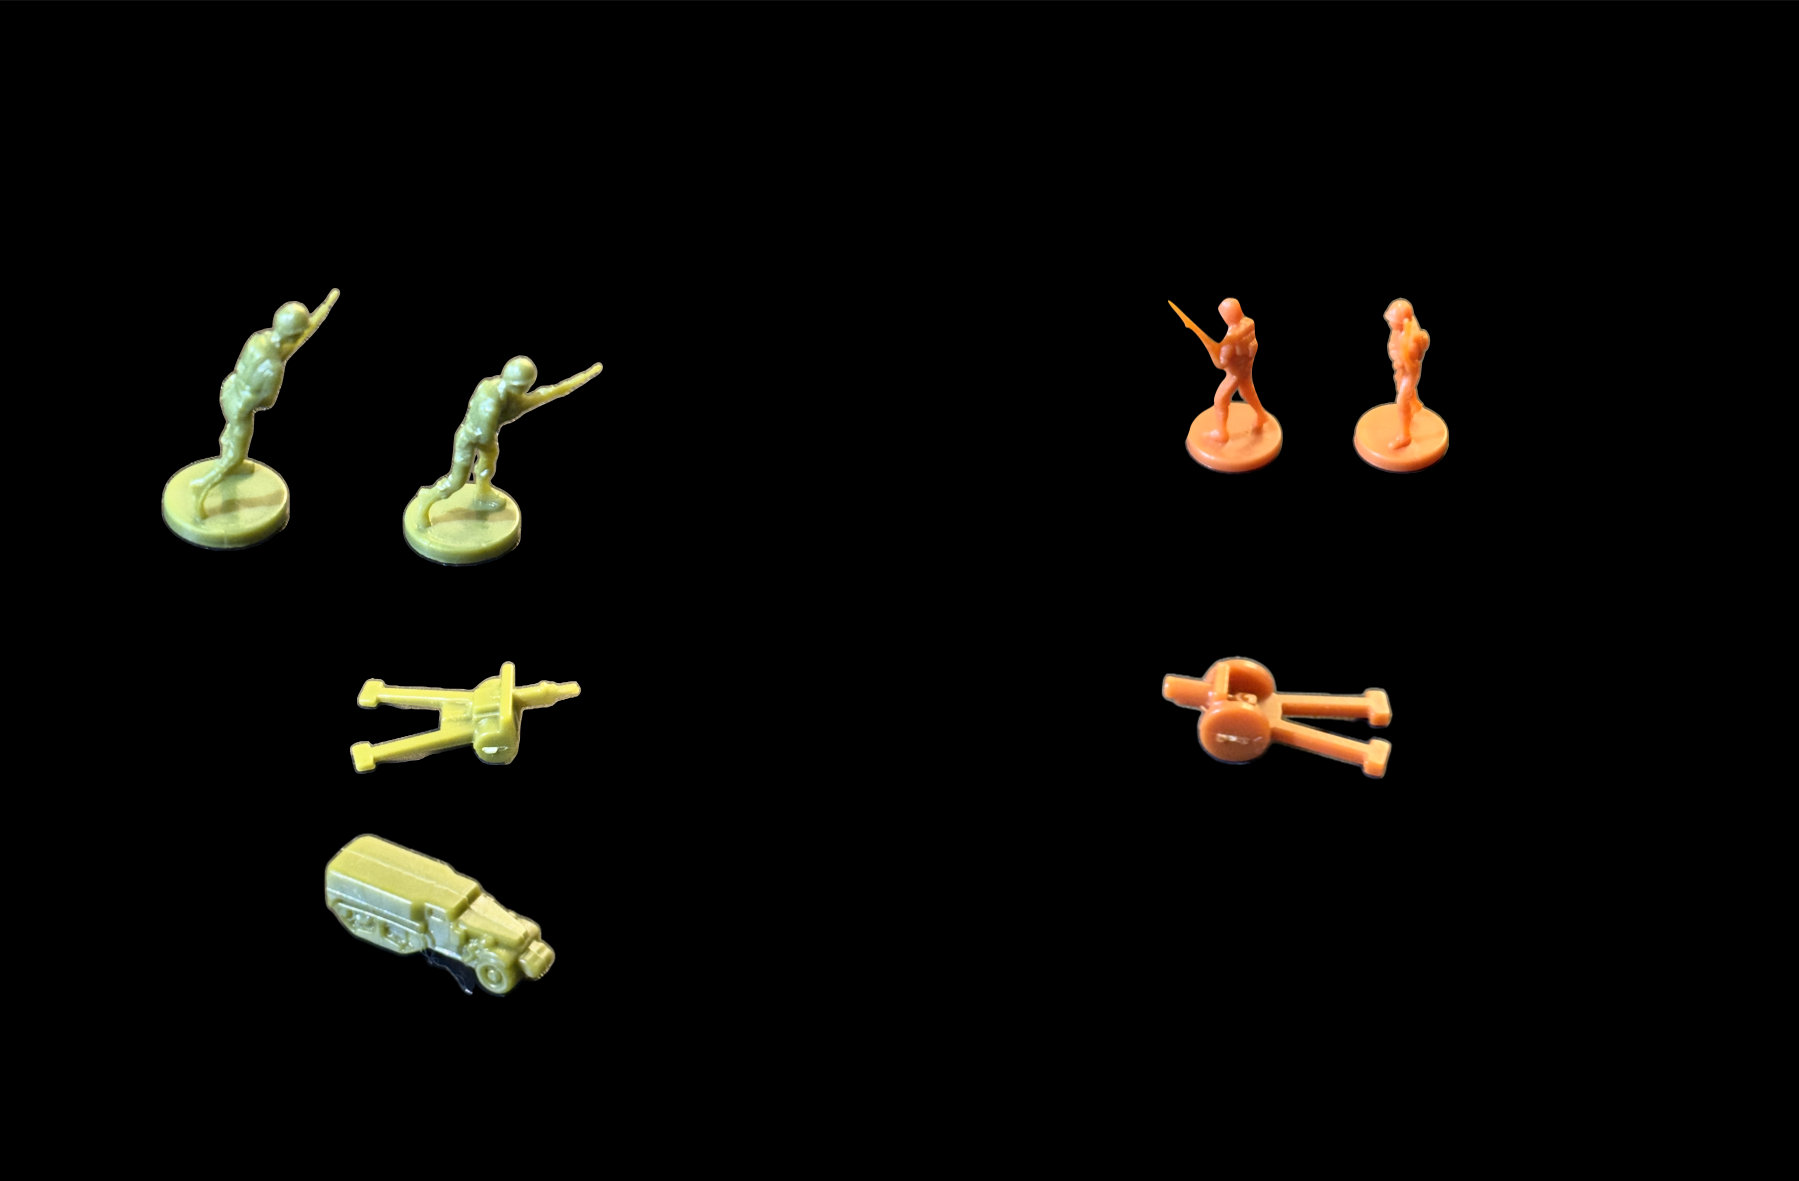
\includegraphics[width=\linewidth]{figures/board_example.jpg}
  \caption{Representative held-out evaluation photograph from
    \texttt{app/backend/test/}. The thirteen images in this directory
    span varying camera angles, lighting conditions, and territory
    layouts; they are the only real-world data the perception
    pipeline is evaluated against and are kept disjoint from any data
    used to fine-tune the ViT classifier.}
  \label{fig:data_example}
\end{figure}

% ============================================================
\section{Method}
\label{sec:method}

\paragraph{Scope refinement from the original proposal.}
The project proposal framed perception as a single whole-board
encoder (a Vision Transformer compared against a CNN baseline)
producing a spatial feature map of the entire game state.
During implementation we found that an \emph{open-vocabulary
detector followed by per-piece classification} was both faster to
develop and better suited to the available data: it requires no
manual bounding-box annotation, generalises across board layouts and
camera angles, and exposes intermediate unit counts that the user
can audit and edit before downstream reasoning runs.
We therefore pivoted the perception stage to the two-step pipeline
described below; the proposed CNN-vs-ViT comparison is retained as a
planned classifier-level ablation
(Section~\ref{sec:planned-eval}).
The downstream reasoning stack (Monte-Carlo simulator $\rightarrow$
MLP win-rate predictor $\rightarrow$ composition recommender) is
unchanged from the proposal; the proposed Bayesian linear-regression
layer (Section~\ref{sec:blr}) has been prototyped offline as part of
the feasibility study, but is not yet wired into the deployed
\texttt{/recommend} path, which currently exhausts the MLP directly.
A second smaller scope simplification is the choice of frontend
technology: the proposal called for a React single-page app, but the
deployed UI is a static HTML page that talks to the FastAPI backend
directly; the React rewrite is treated as future engineering work and
not as a research contribution.

The system is a sequential pipeline of five stages
(Figure~\ref{fig:overview}) operating on the eight-class unit
vocabulary in Table~\ref{tab:units}, which encodes the official cost
and dice statistics from the rulebook.
Of the eight unit types, seven appear on the attacking side; the
anti-aircraft (\textsc{aa}) gun is defender-only by the rules.
Detection and classification therefore work over the seven
attacker-eligible classes, while the simulator and MLP both consume
the full eight-class vocabulary --- which is why the MLP input vector
is fifteen-dimensional (seven attacker counts plus all eight defender
counts).

\begin{table}[h]
\centering\small
\caption{Unit vocabulary modelled by the system. Attack and defence
values are out of six (\emph{Axis \& Allies} uses d6 dice).
\textsc{AA} is defender-only.}
\label{tab:units}
\begin{tabular}{llrc}
\toprule
Code & Unit & IPC & Atk\,/\,Def \\
\midrule
\texttt{Infantry}  & Infantry             &  3 & 1\,/\,2 \\
\texttt{Mech}      & Mechanised infantry  &  4 & 1\,/\,2 \\
\texttt{Artillery} & Artillery            &  4 & 2\,/\,2 \\
\texttt{Tank}      & Tank                 &  6 & 3\,/\,3 \\
\texttt{Fighter}   & Fighter aircraft     & 10 & 3\,/\,4 \\
\texttt{TacBmb}    & Tactical bomber      & 11 & 3\,/\,3 \\
\texttt{StrBmb}    & Strategic bomber     & 12 & 4\,/\,1 \\
\texttt{AA}        & Anti-aircraft gun    &  5 & ---\,/\,1 \\
\bottomrule
\end{tabular}
\end{table}

\subsection{Detection (open-vocabulary)}
\label{sec:detect}

We query OWL-ViT large with seven natural-language prompts, one per
attacker unit family; \textsc{aa} guns are omitted because the rules
forbid the attacker from bringing them, so on a typical board
photograph they are present only on the defending side and do not
need a dedicated detection class.
Detections below confidence $\tau{=}0.05$ are discarded; the remainder
are passed through (a)~NMS at IoU $0.1$, (b)~a containment filter that
removes boxes fully enclosed by a higher-scoring neighbour, and (c)~area
and aspect-ratio sanity checks
($0.001 \leq A_{\text{box}}/A_{\text{img}} \leq 0.4$,
$\text{AR} \leq 10$).

\subsection{Classification (fine-tuned ViT)}
\label{sec:classify}

Each surviving bounding box is cropped, resized to $224{\times}224$,
and normalised with ImageNet statistics before being passed through
a \texttt{vit\_small\_patch16\_224} backbone with a custom 7-way
linear head.
Predictions below confidence $0.7$ are discarded.

\subsection{Faction Assignment (HSV heuristic)}
\label{sec:faction}

Each accepted crop is converted to HSV colour space.
Pixels in the Japan-orange band
($H\!\in\![5,20]$, $S\!\in\![100,255]$, $V\!\in\![100,255]$)
and the USA-green band
($H\!\in\![25,45]$, $S\!\in\![40,255]$, $V\!\in\![40,255]$)
are counted; the piece is assigned to the faction with the
larger count.
This five-line OpenCV~\cite{opencv} step needs no learnable
parameters.
Pieces in any other colour (UK, ANZAC, and China use distinct paint
schemes in the full game) fall outside both HSV bands and are
silently dropped, so the current system scope is Japan vs.\ United
States combat only.

\subsection{Win-Rate Prediction (MLP surrogate)}
\label{sec:mlp}

The 15-dimensional unit-count vector defined in
Section~\ref{sec:method} is fed to a small MLP whose sigmoid output
estimates $P(\text{attacker wins})$.
The network has four fully-connected hidden layers
(widths $256\!\to\!256\!\to\!128\!\to\!64$); the first three layers
are followed by batch normalisation~\cite{batchnorm} and ReLU, the
fourth by ReLU only, and a final \mbox{$64\!\to\!1$} linear head
produces the logit.
We train against binary cross-entropy with
AdamW~\cite{adamw} (lr~$=\!10^{-4}$, weight decay $0.05$) for
$70\,000$ training iterations
on the simulator-generated dataset described in
Section~\ref{sec:data}.
Input features are standardised with training-set statistics that are
saved alongside the weights, so inference uses identical
normalisation.

\subsection{Best-Composition Recommendation}
\label{sec:recommend}

Given a fixed defender stack and budget $B$, we enumerate every
attacker mix with total IPC cost $\leq B$.
With unit costs in $\{3, 4, 4, 6, 10, 11, 12\}$ IPC and budgets
in the low double digits, the candidate set is $O(10^4)$ per budget.
The deployed implementation scores each candidate with a separate
forward pass through the MLP, which is the dominant latency cost in
\texttt{/recommend} (Section~\ref{sec:profiling}); the top-scoring
mix is returned.
The recommender runs twice per request, at two semantically distinct
budgets: once at the \emph{attacker's} own IPC value (answering
\emph{``what should I have brought to this fight for the same money?''})
and once at the \emph{defender's} IPC value
(\emph{``if I matched their investment, what is optimal against this
stack?''}).

\subsection{Bayesian Composition Ranking (prototyped, not deployed)}
\label{sec:blr}

The deployed recommender exhausts the MLP and returns a single
top-scoring mix as a point estimate.
To provide \emph{calibrated} ranking with explicit uncertainty, in the
spirit of weight-uncertainty work for neural
networks~\cite{blundell2015weight}, we have additionally prototyped a
Bayesian linear regression (BLR) head distilled from the trained MLP.
The BLR operates on a hand-crafted $28$-dimensional feature map of
unit counts, force ratios, and pairwise unit-interaction terms; it is
fit online from sufficient statistics, so that adding samples does not
require re-training, and its posterior over compositions is sampled by
Monte Carlo to produce an upper-confidence acquisition score.
On a held-out evaluation set the BLR matches MLP accuracy while running
in $<\!1\,$ms per query on CPU, which lowers the cost of recommendation
search from the MLP-direct baseline ($\sim\!10^{4}$ exhaustive
evaluations, $\sim\!5.6\,$s per budget; see
Section~\ref{sec:profiling}) to evaluating $N\!=\!8\,000$ sampled
candidate mixes in well under one second.
\red{The remaining work --- swapping the BLR into the FastAPI
\texttt{/recommend} endpoint in place of the MLP-direct exhaustive
search, and reporting calibration of the upper-confidence ranking on
the held-out board photos --- is the headline modelling deliverable
for the final submission.}

\subsection{Combat Simulation (rules-based)}
\label{sec:sim}

A deterministic simulator implements the official single-territory
combat sequence in three phases.
\emph{(i)~AA fire} occurs once at the start: each defending AA gun
rolls up to three shots (capped at the number of attacking aircraft)
at $1/6$ to hit, with casualties drawn from fighters, then tactical
bombers, then strategic bombers.
\emph{(ii)~Combat rounds} repeat until one side is wiped: both sides
roll simultaneously at the attack/defence values in
Table~\ref{tab:units}; artillery upgrades paired infantry from $1$
to $2$, and a tactical bomber gains $+1$ when accompanied by a
fighter or tank.
Casualties are applied land-first then air in the order
infantry $\to$ artillery $\to$ tank $\to$ fighter $\to$ tac bomber
$\to$ strategic bomber, with mechanised infantry merged into the
infantry pool for casualty selection and split back out for the
survivor report.
\emph{(iii)~Termination} occurs when one side has no remaining land
or air units.
The RNG is seeded (\texttt{numpy.random.default\_rng(42)}) for
reproducibility.
The simulator is fully vectorised in NumPy~\cite{numpy} and processes
$B\!=\!2\,000$ parallel battles per call, which is what makes the
$100\,000$-sample MLP training set tractable on CPU.
It serves both the user-facing \texttt{/simulate} endpoint
(single-battle deterministic mode) and the win-rate MLP's training-data
generator (high-throughput batched mode).

\begin{figure}[t]
  \centering
  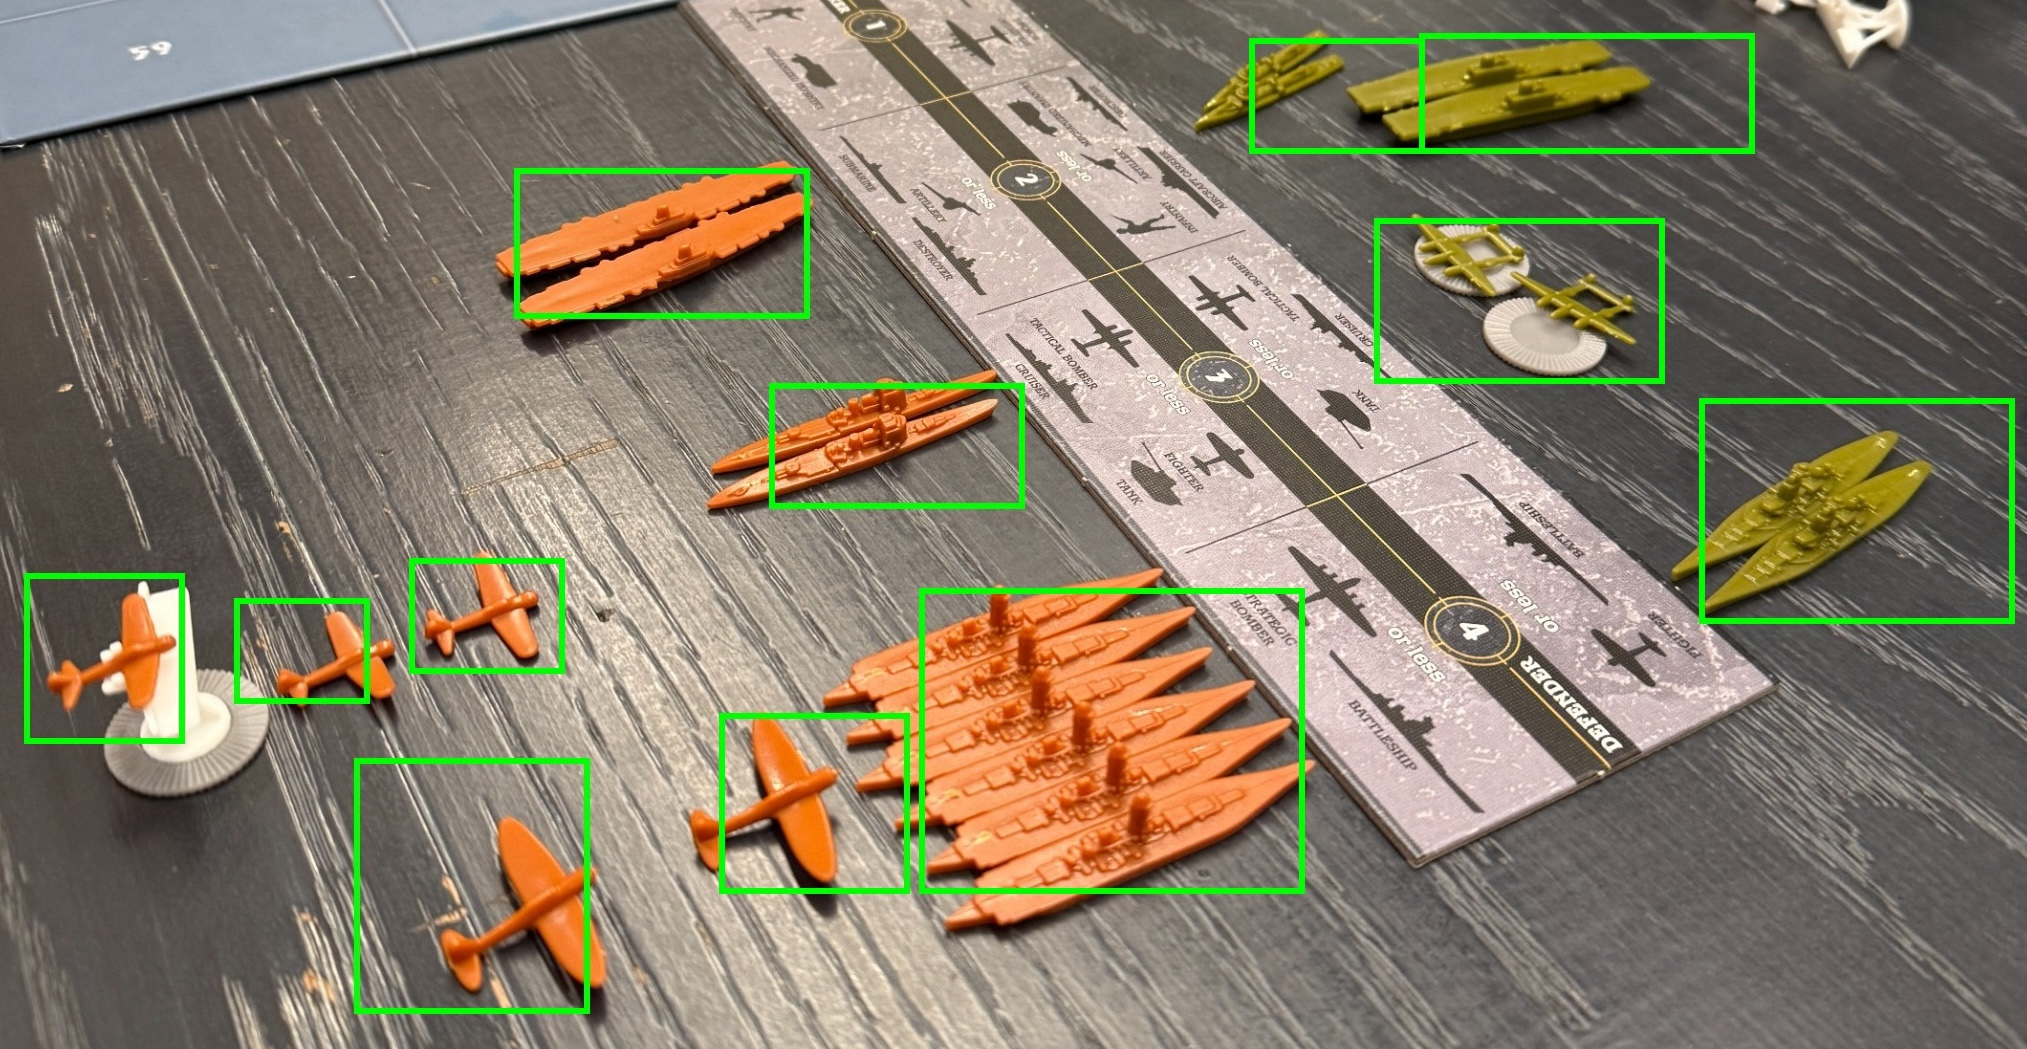
\includegraphics[width=\linewidth]{figures/detection_example.jpg}
  \caption{OWL-ViT detection on a held-out board photograph.
    Each green box is a high-confidence proposal kept after
    NMS, the containment filter, and the area / aspect-ratio sanity
    checks of Section~\ref{sec:detect}; each surviving box is
    forwarded to the ViT classifier (Section~\ref{sec:classify}) and
    the HSV faction step (Section~\ref{sec:faction}).}
  \label{fig:method_detection}
\end{figure}

% ============================================================
\section{Experiments}
\label{sec:experiments}

\subsection{Inference Profiling (complete)}
\label{sec:profiling}

We built a micro-benchmark script
(\texttt{app/backend/bench\_inference.py}) and measured wall-clock
time for each pipeline stage on a Windows CPU laptop
(Table~\ref{tab:latency}).

\begin{table}[h]
\centering
\small
\caption{Per-stage CPU latency (Windows laptop, no GPU).}
\label{tab:latency}
\begin{tabular}{lrl}
\toprule
Stage & Latency & Notes \\
\midrule
OWL-ViT detection     & $\sim$5.0\,s   & Dominates \texttt{/analyze} \\
ViT classification    & $\sim$130\,ms  & Sequential; 1.5$\times$ faster batched \\
MLP single forward    & $\sim$0.28\,ms & Used by \texttt{/winrate} \\
MLP batch (10\textsuperscript{4}) & $\sim$3.8\,ms & $\approx$700$\times$ MLP-only kernel speed-up \\
\texttt{find\_best\_attack} & $\sim$2.8\,s/budget & 2 budgets per \texttt{/recommend} \\
\bottomrule
\end{tabular}
\end{table}

The dominant bottleneck in \texttt{/recommend} is the sequential MLP
calls inside \texttt{find\_best\_attack}.
At the network level, batching all $10^{4}$ candidates into a single
forward pass shrinks the MLP-only cost from $\sim\!2.8$~s to
$\sim\!3.8$~ms (a $\sim\!700{\times}$ kernel-level speed-up); at the
endpoint level the user-visible \texttt{/recommend} call drops from
$\sim\!5.6$~s to under $50$~ms (a $\sim\!112{\times}$ wall-clock
improvement) once the surrounding two-budget loop is included.
Beyond this single fix, our profiling work also identifies a
prioritised optimisation roadmap covering OWL-ViT text-embedding
caching across requests, input-image downscaling before detection,
batched ViT classification of all crops in a single forward, and
\texttt{asyncio} offload of the synchronous \texttt{/analyze} pipeline
so the FastAPI event loop is not blocked for the full inference
window.
We treat that roadmap as an engineering output of the midterm in its
own right; concrete before/after numbers will appear in the final
report.

\subsection{Planned Evaluations \planned}
\label{sec:planned-eval}
\red{Four further evaluations remain for the final submission, all
sharing the same protocol (compute the metric on the held-out
\texttt{app/backend/test/} photographs and crops, then report
alongside the calibration numbers above).
\textbf{Detection accuracy}: hand-label bounding boxes on the
$13$~held-out board photos and report
precision / recall at the operating threshold $\tau\!=\!0.05$,
plus a precision-recall curve and an ablation across OWL-ViT-base,
OWL-ViT-large, and OWLv2~\cite{owlv2}.
\textbf{Classifier accuracy}: per-class top-1 accuracy, macro-F1, and
a confusion matrix on a held-out crop set, highlighting the likely
error pairs (TacBmb vs.\ StrBmb; Mech vs.\ Infantry).
\textbf{CNN vs.\ ViT ablation} (per the original proposal): train a
ResNet-18 baseline on the same crops and compare top-1 accuracy,
parameter count, and CPU latency.
\textbf{Recommendation quality}: for each held-out board, run
\texttt{/recommend} and simulate $10^{3}$ battles for both the
original and recommended attacker mix, reporting the win-rate delta
and the fraction of cases where the recommendation strictly improves
over the original.}

\subsection{Win-Rate Calibration (preliminary)}
\label{sec:winrate-calib}
We evaluated the trained MLP on $500$ held-out battle scenarios drawn
from the same stratified distribution as the training set, using
$5\!\times\!10^{4}$ simulator rollouts per scenario as the ground-truth
win rate.
The mean absolute error is $\mathrm{MAE} = 0.0034$, i.e., the model
deviates from the simulator by roughly $0.34$ percentage points on
average across the test set.
Table~\ref{tab:mlp-rep} reports four representative scenarios spanning
small / balanced / asymmetric force compositions; in each case the
MLP tracks the simulator within half a percentage point.
\red{A reliability diagram and per-stratum breakdown
($[0,3]$ vs.\ $[0,10]$ vs.\ $[0,30]$) will appear in the final report.}

\begin{table}[h]
\centering\small
\caption{MLP win-rate prediction vs.\ Monte-Carlo simulator on
representative battles.}
\label{tab:mlp-rep}
\begin{tabular}{lcc}
\toprule
Scenario & Simulator & MLP \\
\midrule
1 inf vs 1 inf                         & 0.417 & 0.421 \\
1 inf {+} 1 art vs 1 inf {+} 1 art     & 0.500 & 0.497 \\
1 tank vs 1 inf                        & 0.782 & 0.779 \\
3 inf {+} 1 art {+} 1 tank vs same     & 0.500 & 0.503 \\
\bottomrule
\end{tabular}
\end{table}

\begin{figure}[t]
  \centering
  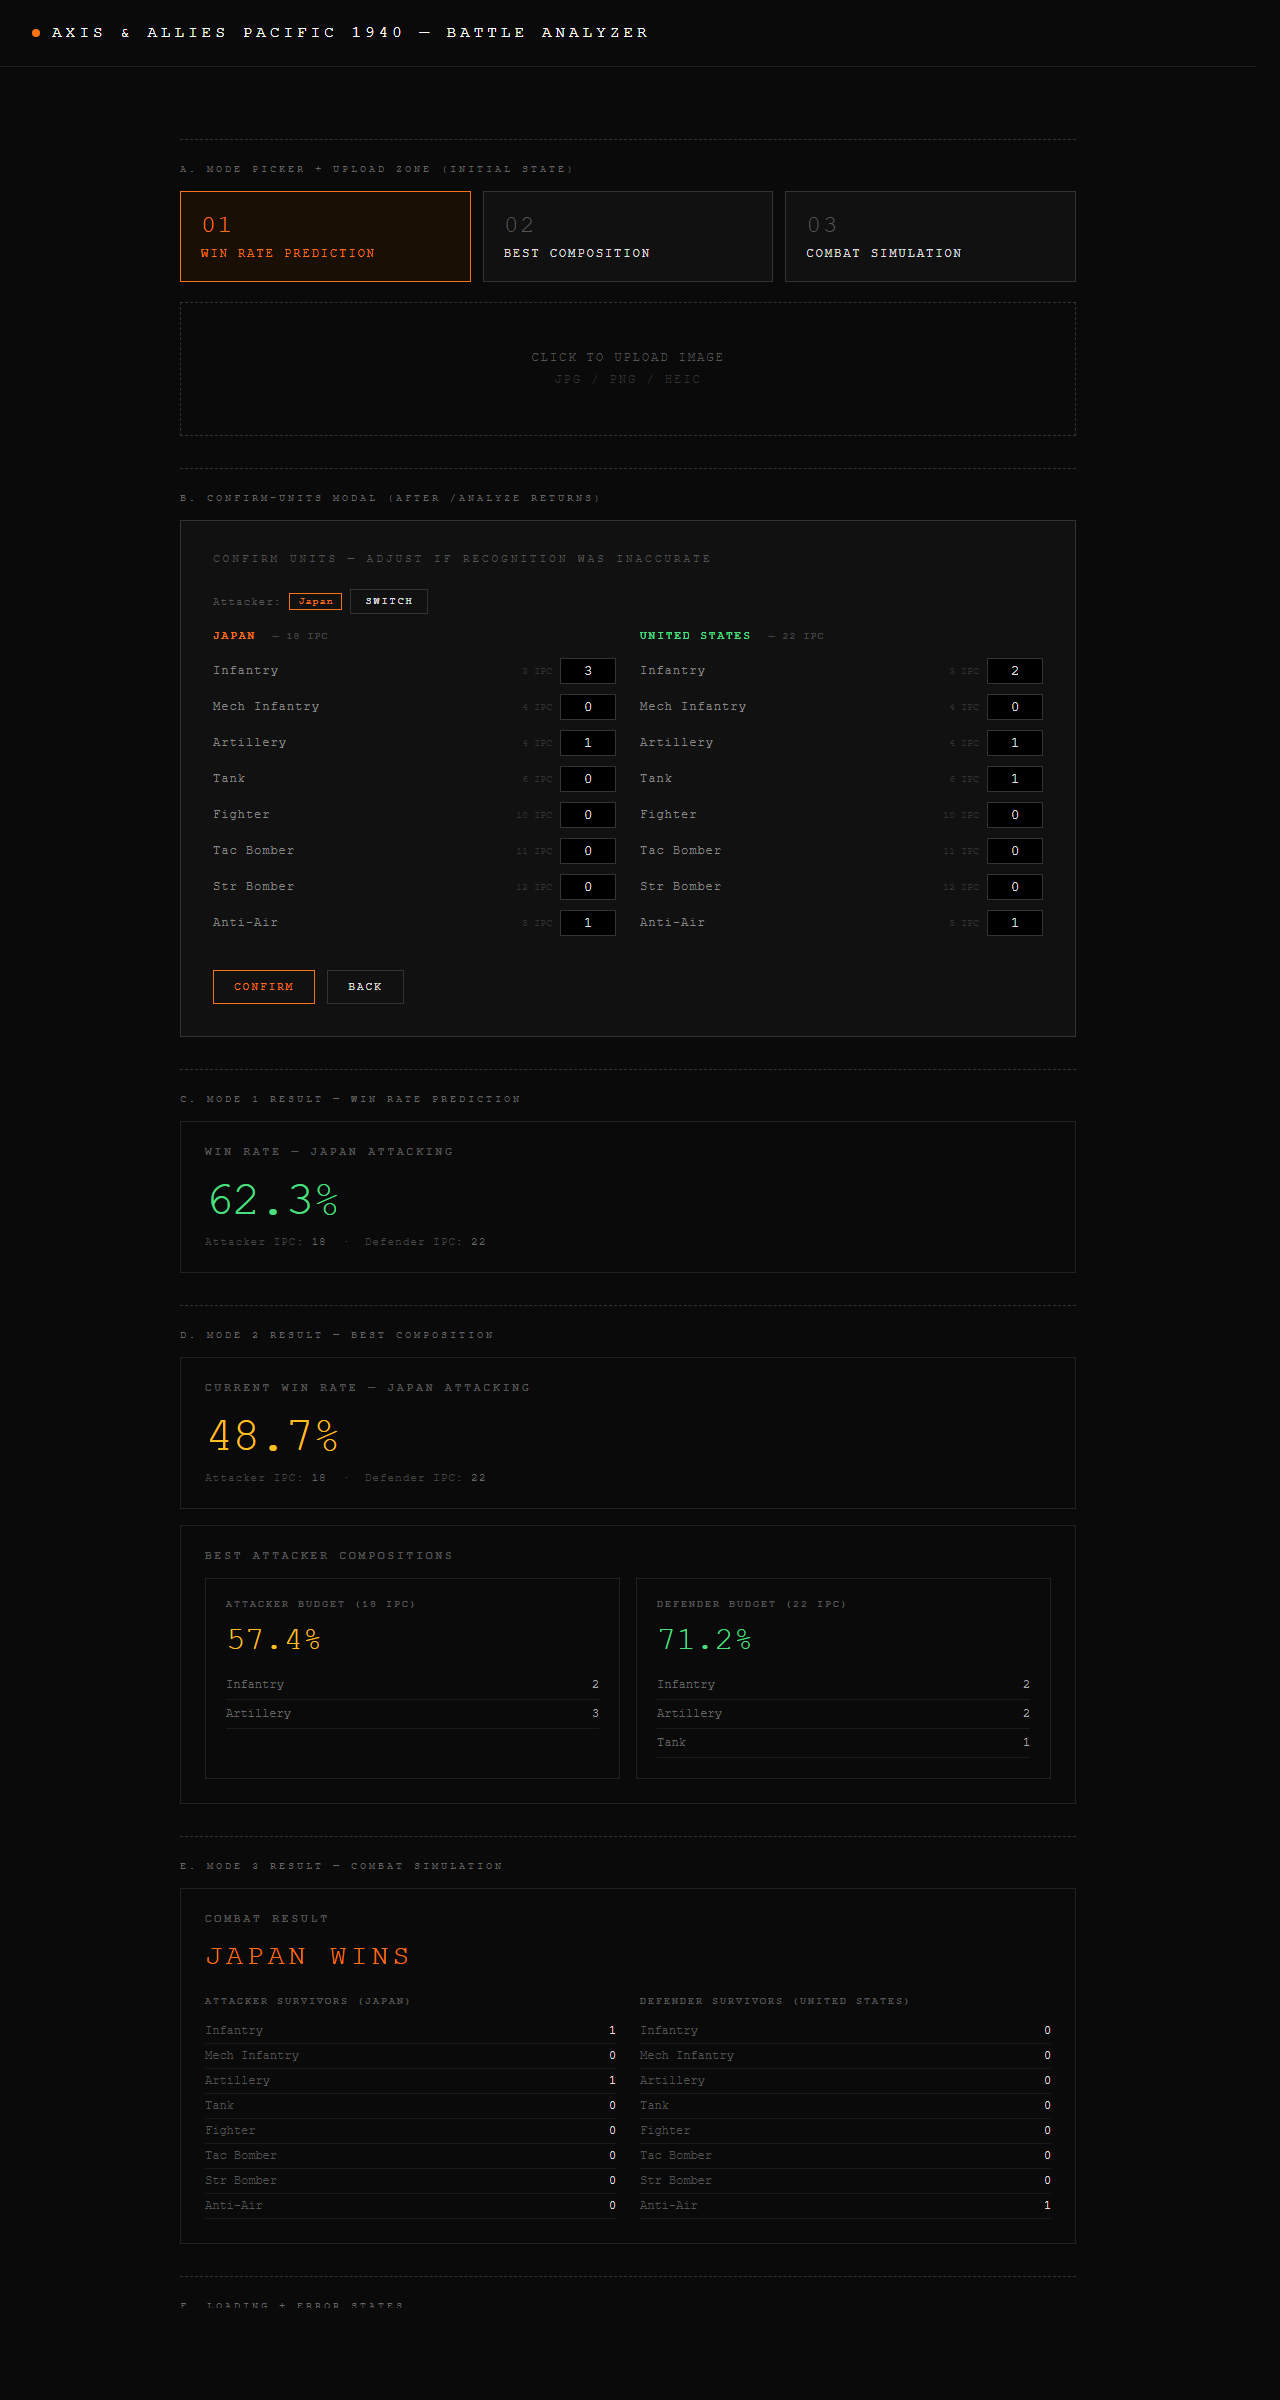
\includegraphics[width=\linewidth]{figures/ui_states.png}
  \caption{End-to-end system output captured against the deployed
    FastAPI backend. Top: the confirm-units modal that follows
    \texttt{/analyze}. Middle row, left to right: the
    Win-Rate Prediction panel (Mode~1, Section~\ref{sec:mlp}), the
    Best-Composition recommendation cards (Mode~2,
    Section~\ref{sec:recommend}), and the Combat-Simulation result
    panel (Mode~3, Section~\ref{sec:sim}). Bottom: loading and error
    states. The same composite is the basis for the UX audit
    referenced in Section~\ref{sec:conclusion}.}
  \label{fig:experiments}
\end{figure}

% ============================================================
\section{Conclusion and Future Work}
\label{sec:conclusion}

We have demonstrated a functioning end-to-end pipeline that converts
a phone photograph of a board-game position into three forms of
tactical decision support.
The perception and serving infrastructure are complete and verified
across macOS, Linux, and Windows.
\red{Remaining work concentrates on (i)~quantitative evaluation of
the individual perception stages on the held-out board photographs,
(ii)~batching the MLP scoring loop to bring \texttt{/recommend} from
$\sim$5.6\,s to under $50$\,ms ($\sim\!112{\times}$ user-visible
speed-up), (iii)~swapping the prototyped BLR ranker into the
production \texttt{/recommend} path in place of MLP-direct exhaustive
search, and (iv)~a user study comparing player decisions with and
without the tool.}

\paragraph{What we built vs.\ what we leveraged.}
The OWL-ViT detector~\cite{owlvit} weights and the
\texttt{transformers} library~\cite{hftransformers} are used unchanged
from public releases; the ViT-Small backbone is the unmodified
\texttt{vit\_small\_patch16\_224} from \texttt{timm}~\cite{timm}, with
only the seven-class linear head, the seven OWL-ViT text prompts, and
the fine-tuning recipe being ours.
Every other component --- the HSV faction-colour heuristic, the
win-rate MLP architecture and its training pipeline, the rules-based
combat simulator, the exhaustive IPC-budget recommender, the FastAPI
service, and the static HTML frontend --- was implemented from scratch
in this project.

\paragraph{Engineering effort beyond modelling.}
Three pieces of system work are claimed for credit alongside the
modelling.
First, a two-phase setup audit on a clean Windows host produced a
README rewrite, surfaced three dependencies missing from
\texttt{requirements.txt} (\texttt{transformers},
\texttt{python-multipart}, \texttt{matplotlib}), and identified two
runtime bugs in the existing code base
(defender-Mech survivor accounting in the combat simulator and an
\texttt{AA}-field omission in the \texttt{/recommend} payload).
Second, a microbenchmark harness was written from scratch to
characterise per-stage CPU latency
(Table~\ref{tab:latency}); it both isolated the
\texttt{find\_best\_attack} bottleneck and quantified the headroom
available from batching.
Third, a UX audit captured all six dynamic frontend states under
headless Edge and produced a prioritised list of seventeen
friction-and-gap items, including the \texttt{file://} CORS issue
that originally blocked first-time users from completing an upload.

% ============================================================
{\small
\bibliographystyle{ieeenat_fullname}
\bibliography{references}
}

\end{document}
